\documentclass[xcolor={table}]{beamer}
\usepackage{./sty/beamerthemeMSU}
\usepackage{verbatim}

% Packages
%\usepackage{caption}
\usepackage{hyperref}
%\usepackage{media9}   % If embedding sound/video
\usepackage{amsmath} % Used on formula slide

\usepackage{cancel}     % Used on formula slide
\usepackage{listings}    % If using syntax highlighting
%\input{./code/csci112_listings.tex}
\usepackage{tikz}	       % If using tikz
\usepackage{algorithmic}
\usepackage{algorithm}
\usepackage{graphicx}
\graphicspath{ {sty/} }
\usepackage{graphicx}
\newcommand{\R}{\mathbb{R}}
%added these in, might not always need
\usepackage{multicol}
\newcommand{\dataset}{{\cal D}}
\newcommand{\fracpartial}[2]{\frac{\partial #1}{\partial  #2}}
\newcommand{\argmax}{\arg\,\max}
%\newtheorem{theorem}{theorem}
%\newtheorem{lemma}[theorem]{Lemma}
% Miscellaneous control settings
\setlength{\columnsep}{1cm}

\title[TD($\lambda$)]{Robustness May Be at Odds with Accuracy}
\author[Pan and Yang]{Dimitris Tsipras, Shibani Santurkar, Logan Engstrom,
Alexander Turner, Aleksander Madry}
\date{February 27, 2020}

%%%%%%%%%%% Title %%%%%%%%%%%%
\begin{document}
\begin{frame}
  \maketitle
\end{frame}

%%%%%%%%%%% Intro %%%%%%%%%%%%
\begin{frame}{The Motivation For Transfer Learning}
    \begin{itemize}
        \item Many machine learning algorithms work well under the assumption that training and test data are drawn from the same feature space and same distribution.
        \item In the real world if the distribution changes it can be difficult to recollect data and build new models.
        \item Transfer learning allows domains, tasks, and distributions used in training and testing to be different.
        \item Authors give the example of sentiment analysis in the context of classifying product reviews.
        \item That humans are capable of applying knowledge gained from past tasks to solve new problems, further motivates the study of transfer learning.
    \end{itemize}
\end{frame}

\begin{frame}{Formal Definition of Transfer Learning}
    \begin{itemize}
        \item \textit{Forward View} - estimate at each time step is moved toward an update target known as $\lambda-return$ ($\lambda-return$ algorithm)
        \item $\lambda-return$ - estimate of the expected return based on both the subsequent rewards and the expected return estimates at subsequent states, where $\lambda$ determines the precise way of combining these.
        \item Not clear how $\lambda-return$ could form a basis for online algorithm.
        \item Estimates are not updated every step
        \item $\lambda-return$ is most often not known till the end of episode
        \item TD($\lambda$)- each step only requires temporally local info $->$ can be online%immediate next reward and next state
        \item Updates occur during episode in the online version
        \item Online TD($\lambda$) will not equal $\lambda-return$ in the end
    \end{itemize}
\end{frame}

\begin{frame}{Problem Setting}
    \textbf{Markov Reward Processes}
    \begin{itemize}
        \item 4-tuples - $\langle\mathcal{S},p,r,\gamma\rangle$
        \item $\mathcal{S}$ - state space
        \item $p(s'|s)$ - transition probability function
        \item $r(s,s')$ - reward function
        \item $\gamma$ - discount factor %how future rewards are weighted w.r.t. immediate reward
    \end{itemize}
    Return at time step \textit{t} (discounted sum of rewards after \textit{t}):
    \begin{equation*}
        G_{t} = \sum_{i=1}^{\infty } \gamma^{i-1}R_{t+i}
    \end{equation*}
\end{frame}

\begin{frame}{Problem Setting Cont.}
    \begin{itemize}
        \item MRPs can have \textit{terminal states} that divide the sequence of state transitions into \textit{episodes}.
        \item When reaching terminal state, the current episode ends and state is reset to initial state
    \end{itemize}
    Return for an episodic MRP :
    \begin{equation*}
        G_{t} = \sum_{i=1}^{T-t } \gamma^{i-1}R_{t+i}
    \end{equation*}
    where \textit{T} is the time step the terminal state is reached.
    \begin{equation*}
        v(s) = \mathbb{E}\left \{ G_{t} | S_{t} = s \right \}
    \end{equation*}
    Value-function \textit{v} maps each state to expected value of return
\end{frame}

\begin{frame}{Problem Setting Cont.}
    \textbf{Function Approximation}
    \begin{itemize}
        \item Function approximation used to represent \textit{v}
        \item $\hat{v_{t}}(s,\boldsymbol{\theta})$ - approximate value of state \textit{s}, given weight vector $\boldsymbol{\theta}$.
        \item Linear function approximation -  value of state is the inner product between the weight vector $\boldsymbol{\theta}$ and state-dependent feature vector $\boldsymbol{\phi}(s)$:
           \begin{equation*}
               \hat{v_{t}}(s) = \boldsymbol{\theta_{t}^{T}}\boldsymbol{\phi}(s) = \sum_{i}\theta_{i,t}\phi_{i}(s)
           \end{equation*}
        \item Gradient to update weight vector $\boldsymbol{\theta}$ at each time step in direction of gradient of time step's error:
        \begin{equation*}
            \boldsymbol{\bigtriangledown}_{\boldsymbol{\theta}_{t}}\hat{v}_{t}(S_{t}) = \boldsymbol{\phi}_{t}
        \end{equation*}
        \item End of episode: weight vector updated by summing all weight corrections:
        \begin{equation*}
            \boldsymbol{\theta}_{k+1} = \boldsymbol{\theta}_{k} + \sum_{t=0}^{T-1}\boldsymbol{\Delta}_{t}
        \end{equation*}
    \end{itemize}
\end{frame}

\begin{frame}{Problem Setting Cont.}
    \begin{figure}
        \centering
        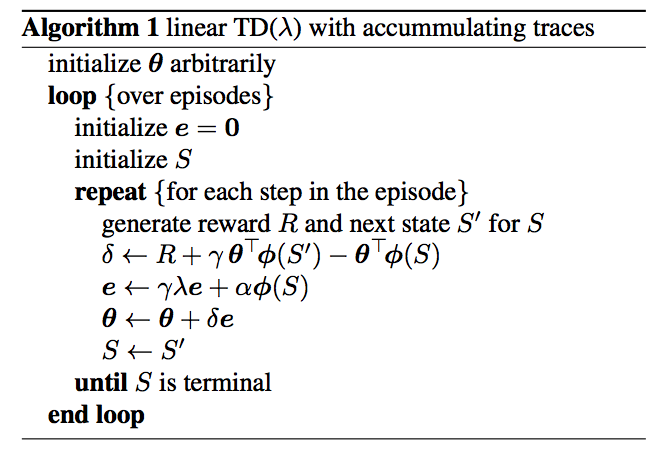
\includegraphics[scale = 0.43]{lineartd.png}
        \label{fig:my_label}
    \end{figure}
\end{frame}

\begin{frame}{Problem Setting Cont.}
    \textbf{The Conventional Forward View}
    \begin{itemize}
        \item Related to $\lambda-return$ algorithm
        \item Performs a standard update at each time step with $\lambda-return$ as update target
        \item $\lambda-return$ $G_{t}^{\lambda}$- estimate of expected return based on combinations of rewards and other estimate:
        \begin{equation*}
            G_{t}^{\lambda} = (1-\lambda)\sum_{n=1}^{\infty }\lambda^{n-1}G_{t,\boldsymbol{\theta}}^{(n)}
        \end{equation*}
        with weight vector $\boldsymbol{\theta}$ corresponding to current episode
        \item $G_{t,\boldsymbol{\theta}}^{(n)}$ \textit{n}=step return:
        \begin{equation*}
            G_{t,\boldsymbol{\theta}}^{(n)} = \sum_{i=1}^{n}\gamma^{i-1}R_{t+i} + \gamma^{n}\boldsymbol{\theta}^{\top}\boldsymbol{\phi}_{t+n }
        \end{equation*}
    \end{itemize}
\end{frame}

\begin{frame}{Problem Setting Cont.}
    \textbf{The Conventional Forward View}
    \begin{itemize}
        \item Episodic task - $\lambda-return$:
        \begin{equation*}
            G_{t}^{\lambda} = (1-\lambda)\sum_{n=1}^{T-t-1}\lambda^{n-1}G_{t,\boldsymbol{\theta}}^{(n)} + \lambda^{T-t-1}G_{t,\boldsymbol{\theta}}^{(T-t)}
        \end{equation*}
        where \textit{T} is the time step that the terminal state is reached
        \item Value of terminal state is always 0, therefore the last \textit{n}-step return equals the full return:
        \begin{equation*}
            G_{t,\boldsymbol{\theta}}^{(T-t)} = \sum_{i=1}^{T-t}\gamma^{i-1}R_{t+i} = G_{t}
        \end{equation*}
        \item Online TD($\lambda$) is only approximately equal to online $\lambda$-return algorithm. Not possible for them to be equal since $\lambda$-return uses future rewards and states
    \end{itemize}
\end{frame}

\begin{frame}{An Online Forward View}
    \begin{itemize}
        \item Goal: Construct version of online TD($\lambda$) that matches forward view exactly
        \item ``Online Learning": the value estimates are updated at every time step, but doesn't rule out using future information
        \item However, online TD($\lambda$) uses only information up to
        time step \textit{t} for update $\rightarrow$ \textit{strict-online}
        \item Let $t'$ be the time step $\lambda$-return is truncated, let $truncated$ $\lambda-return G_{t}^{\lambda|t'}$ be:
        \begin{equation*}
            G_{t}^{\lambda|t'} = (1-\lambda)\sum_{n=1}^{t'-t-1}\lambda^{n-1}G_{t,\boldsymbol{\theta}_{t+n-1}}^{(n)} + \lambda^{t'-t-1}G_{t,\boldsymbol{\theta}_{t'-1}}^{(t'-t)}
        \end{equation*}
    \end{itemize}
\end{frame}

\begin{frame}{An Online Forward View Cont.}
    \begin{itemize}
        \item Idea: At each time step, the truncated $\lambda$-returns from all previous time steps are updated, such that they are now truncated at the current time step.
        \item The weight vector of the current time step is determined by sequentially performing TD backup using the update $\lambda$-returns, starting from initial weight vector $\boldsymbol{\theta}_{init}$
        \item Weight vector $\boldsymbol{\theta}_{t,k}$ is incrementally defined:
        \begin{equation*}
            \boldsymbol{\theta}_{t,k} = \boldsymbol{\theta}_{t,k-1} + \alpha_{k-1}\left [ G_{k-1}^{\lambda|t} - \boldsymbol{\theta}_{t,k-1}^{\top}\boldsymbol{\phi}_{k-1}\right ]\boldsymbol{\phi}_{k-1}
        \end{equation*}
        for $0 < k \leq t$, with $\boldsymbol{\theta}_{t,0} = \boldsymbol{\theta}_{init}$.
        \item Truncated $\lambda$-return is expensive and requires storage of all observed states and rewards.
    \end{itemize}
\end{frame}

\begin{frame}{True Online TD($\lambda$)}
    \begin{itemize}
        \item Implements strict-online forward view efficiently using eligibility trees
        \item Feature weights updated proportionally to decaying eligibility tree
        \begin{figure}
            \centering
            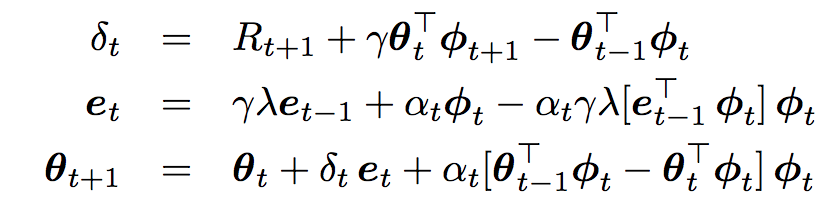
\includegraphics[scale = 0.7]{equation.png}
            \label{fig:my_label}
        \end{figure}
    \end{itemize}
\end{frame}

\begin{frame}{True Online TD($\lambda$) Cont.}
    \begin{figure}
        \centering
        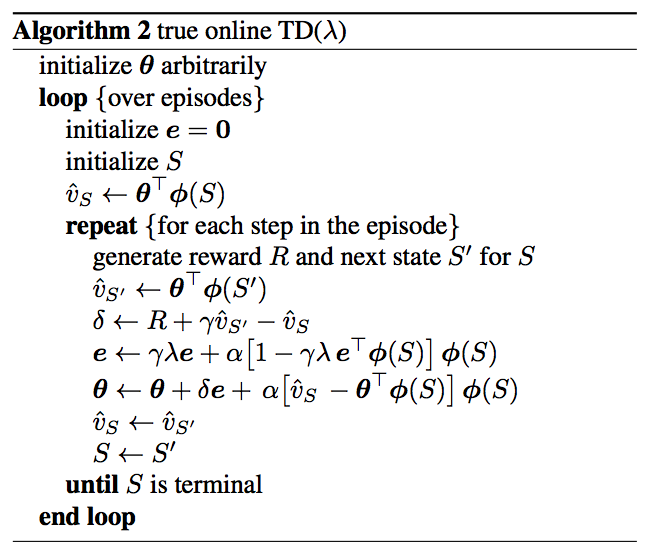
\includegraphics[scale = 0.41]{trueonline.png}
        \label{fig:my_label}
    \end{figure}
\end{frame}

\begin{frame}{Equivalence to the Online Forward View}
    \begin{lemma}
        \textbf{Lemma 1}: $G_{t}^{\lambda|t'}$, used by the truncated $\lambda$-return algorithm, is related to $\delta_{t}$, used by true online  TD($\lambda$), as follows:
        \begin{equation*}
            G_{t}^{\lambda|t'+1} - G_{t}^{\lambda|t'} = (\gamma\lambda)^{t'-t}\delta_{t'}
        \end{equation*}
        \textbf{Lemma 2}:
        The following equation holds:
        \begin{equation*}
            \boldsymbol{\theta}_{t+1,t} - \boldsymbol{\theta}_{t,t} = \gamma\lambda\delta_{t}e_{t-1}
        \end{equation*}
    \end{lemma}
    \begin{theorem}
        $\boldsymbol{\theta}_{t,t}$, computed by the truncated $\lambda$-return algorithm, is the same as $\boldsymbol{\theta}_{t}$, computed by true online TD($\lambda$), for all time steps t.
    \end{theorem}
\end{frame}

\begin{frame}{Empirical Results}
    \begin{figure}
        \centering
        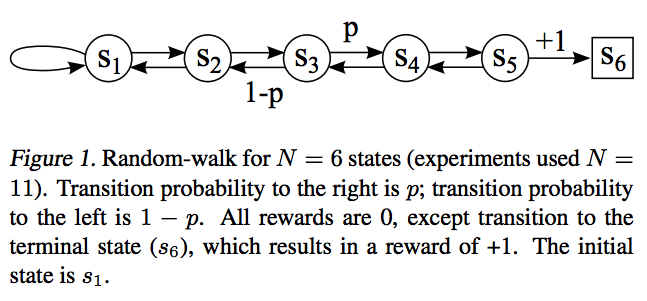
\includegraphics[scale = 0.5]{random-walk.png}
        \label{fig:my_label}
    \end{figure}
\end{frame}



\begin{frame}{Empirical Results Cont.}
    \begin{figure}
        \centering
        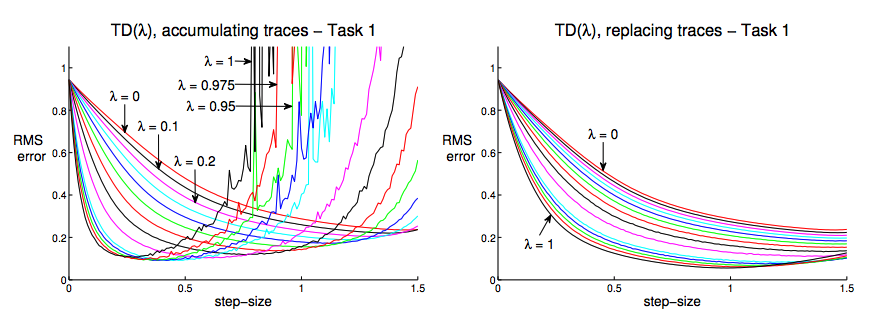
\includegraphics[scale = 0.33]{fig2-1.png}
        \label{fig:my_label}
    \end{figure}
    \begin{figure}
        \centering
        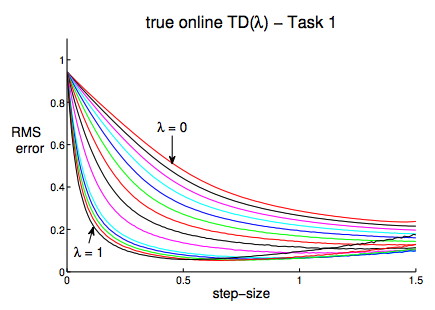
\includegraphics[scale = 0.33]{fig2-2.png}
        \label{fig:my_label}
    \end{figure}
\end{frame}

\begin{frame}{Empirical Results Cont.}
    \begin{figure}
        \centering
        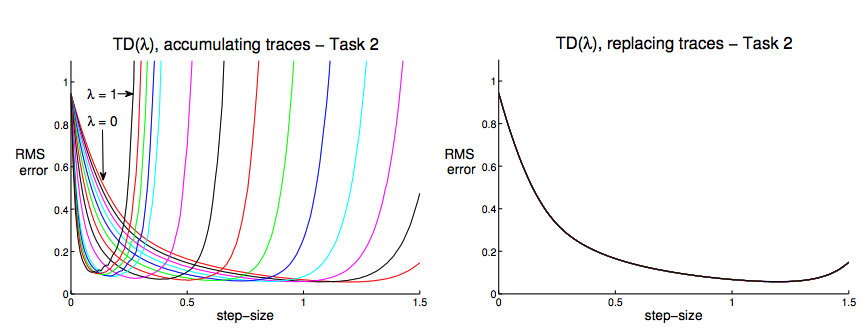
\includegraphics[scale = 0.33]{fig2-3.png}
        \label{fig:my_label}
    \end{figure}
    \begin{figure}
        \centering
        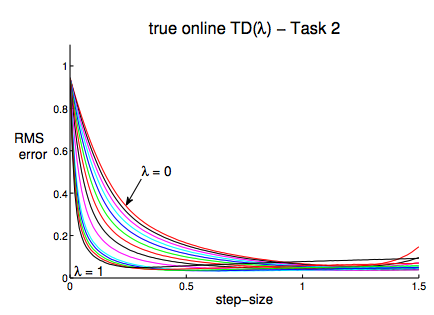
\includegraphics[scale = 0.33]{fig2-4.png}
        \label{fig:my_label}
    \end{figure}
\end{frame}

\begin{frame}{Empirical Results Cont.}
    \begin{figure}
        \centering
        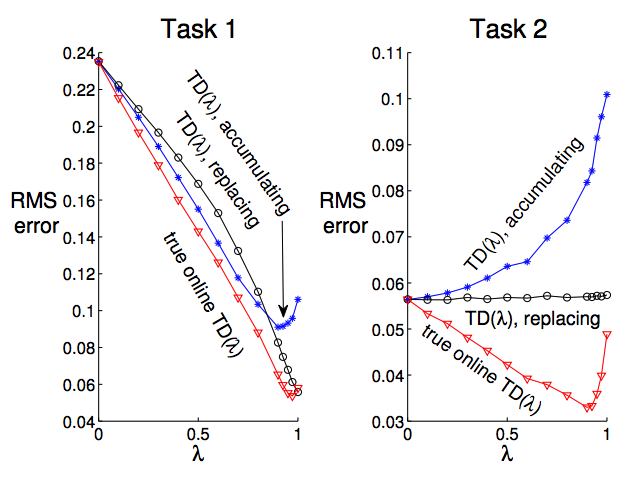
\includegraphics[scale = 0.45]{fig3.png}
        \label{fig:my_label}
    \end{figure}
\end{frame}

\begin{frame}{Control}
    \begin{itemize}
        \item True Online TD($\lambda$) can be modified for control easily.
        \item Use feature vector consisting of state-action features
        \item $\boldsymbol{\phi(s,a)}$ instead of $\boldsymbol{\phi(s)}$
        \item Changes algorithm to true online Sarsa($\lambda$)
        \item Tested on the mountain car problem
        \item Results show true online principle effective in control setting
    \end{itemize}
    \begin{figure}
        \centering
        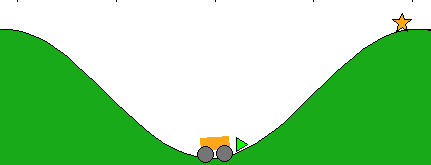
\includegraphics[scale = 0.4]{mountaincar.png}
        \caption{Mountain Car Problem}
        \label{fig:my_label}
    \end{figure}
\end{frame}

\begin{frame}{Control}
    \begin{figure}
        \centering
        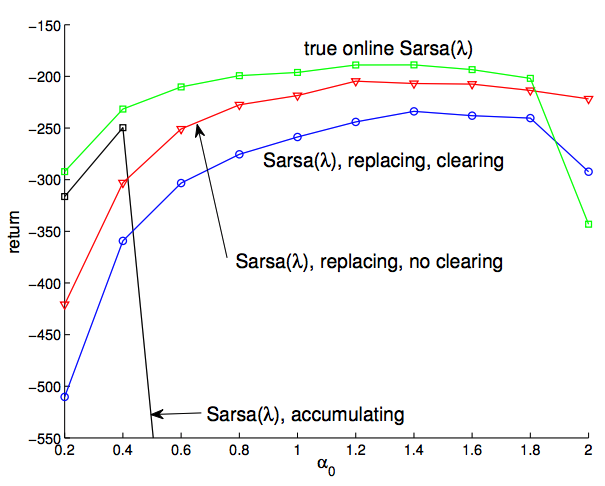
\includegraphics[scale = 0.45]{fig4.png}
        \label{fig:my_label}
    \end{figure}
\end{frame}

\begin{frame}{Conclusion}
    \begin{itemize}
        \item Presented first time online version of forward view \item Forms theoretical and intuitive foundation for TD($\lambda$) algorithm
        \item Developed new variant of TD($\lambda$) with same computational complexity as original, called true online TD($\lambda$)
        \item Proved true online TD($\lambda$) matches new online forward view exactly (classic TD($\lambda$) is only approximate)
        \item True online TD($\lambda$) outperforms other TD($\lambda$) variants on three benchmark problems
        \item Adheres to TD($\lambda$) goal: matching an intuitively clear forward view even in the online case
    \end{itemize}
\end{frame}

\begin{frame}{Discussion Questions}
    \begin{enumerate}
        \item What were the best qualities of the paper?
        \item What did you find the most useful/valuable in the paper?
        \item In your opinion, what was the main contribution of this paper?
        \item Describe a situation where using the classic TD($\lambda$) algorithm would be a better option over the True Online TD($\lambda$) algorithm.
        \item What would you have done differently in regards to the paper?
        \item Explain why the results claimed are/are not valid and significant.
        \item True Online TD($\lambda$) was only compared to other variations of TD($\lambda$).  How do you think True Online TD($\lambda$) would stack up with other reinforcement learning algorithms?
        \item How could the use of the True Online TD($\lambda$) algorithm benefit ongoing research in the lab?
    \end{enumerate}
\end{frame}
\end{document}
